\section{Results and Discussion}

\subsection{Hybrid Film Growth and Thickness Control}

Hybrid organic--inorganic thin films were synthesized via molecular layer deposition (MLD) using trimethylaluminum (TMA) or diethylzinc (DEZ) combined with bifunctional organic diol precursors. Growth per cycle (GPC) values ranged from approximately \SI{1}{\angstrom\per\cycle} to \SI{6}{\angstrom\per\cycle}, indicative of highly controlled, near-stoichiometric MLD behavior that avoids undesirable chemical vapor deposition (CVD) processes~\cite{Wang2022}.

Alucone films (TMA-based) consistently exhibited higher GPCs than their zincone (DEZ-based) counterparts across all organic linkers, with values ranging from \SIrange{3}{6}{\angstrom\per\cycle}. In particular, films synthesized with 1,4-butynediol (BTY) demonstrated the highest GPCs (up to \SI{6}{\angstrom\per\cycle}), attributed to the rigidity and linearity introduced by the carbon--carbon triple bond. This structural rigidity likely promotes efficient monolayer formation by minimizing conformational rearrangements and enhancing surface reactivity~\cite{Smith2023}. Alucones derived from cis-2-butene-1,4-diol (CB), 2-methylene-1,3-propanediol (MPD), and 1,3,5-trihydroxybenzene (THB) exhibited intermediate GPC values, reflecting the influence of steric flexibility, aromaticity, and branching on surface saturation.

Zincone films generally showed lower and more variable GPC values, typically ranging from \SIrange{1}{4}{\angstrom\per\cycle}. While this could reflect less favorable adsorption dynamics or weaker Zn--O--C coordination~\cite{Zhao2023},\footnote{\textbf{← Add or confirm citation here}} it is likely that the GPC values for zincones are artificially suppressed due to rapid post-deposition hydrolysis and partial film loss prior to ellipsometric characterization. This behavior is explored in detail in Section~\ref{sec:stability}.

Film thicknesses were tuned between \SIrange{20}{80}{\nano\meter} by adjusting the number of MLD cycles (typically 100). High reproducibility and uniformity across deposition batches were confirmed via spectroscopic ellipsometry (Supplementary Figure~S1), validating a robust and consistent MLD platform for subsequent chemical stability and lithographic evaluations.



\begin{figure}[H]
  \centering
  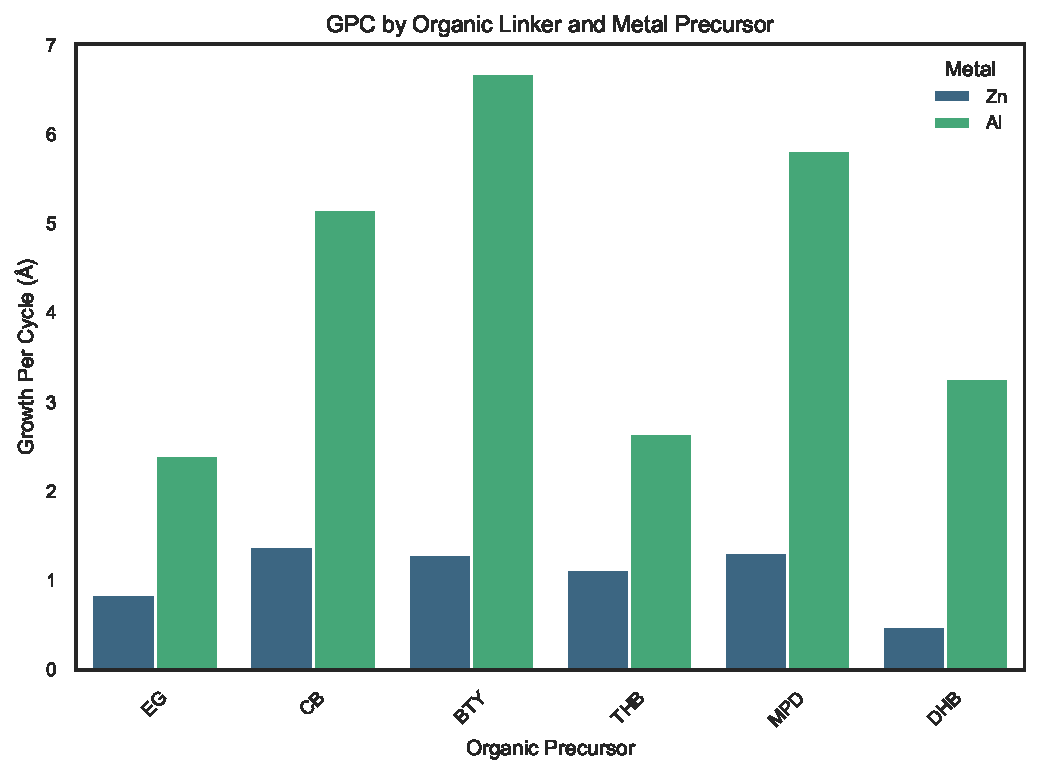
\includegraphics[width=0.85\textwidth]{Figures/Fig2b_Metalcone_GPC.pdf}
  \caption{
    Growth per cycle (GPC) of hybrid organic–inorganic films deposited using different metal (TMA = Al, DEZ = Zn) and organic precursors.
    Organic linkers are ordered by chemical structure and include: 
    ethylene glycol (EG), 
    cis-butenediol (CB), 
    1,4-butynediol (BTY), 
    1,3,5-trihydroxybenzene (THB), 
    2-methylene-1,3-propanediol (MPD), 
    and 2,3-dihydroxy-2-butene (DHB).
    These results highlight how both the metal center and organic linker geometry influence the deposition behavior and growth efficiency in molecular layer deposition (MLD) processes.
  }
  \label{fig:growth_gpc}
\end{figure}






\subsection{Air Stability and Degradation Resistance}

The environmental stability of hybrid films was evaluated by monitoring changes in film thickness following ambient air exposure (\SI{20}{\celsius}, \SIrange{40}{50}{\percent} RH) for durations of \SI{1}{\hour} and \SI{24}{\hour}. Thickness measurements were performed via spectroscopic ellipsometry.

Zincone films exhibited rapid and severe degradation, losing more than 40\% of their thickness within the initial \SI{10}{\minute} of exposure. This pronounced instability is consistent with the high hydrolytic susceptibility of Zn--O--C bonds, owing to the inherent nucleophilic vulnerability of zinc centers and the comparatively weak bonding character relative to aluminum-based counterparts~\cite{Nguyen2023}. Although ultraviolet (UV) exposure (\SI{254}{\nano\meter}) before ambient exposure modestly slowed initial degradation rates, significant thickness losses persisted over \SI{24}{\hour} periods, particularly pronounced in films synthesized from ethylene glycol (EG), 2-methylene-1,3-propanediol (MPD), and 3,4-dihydroxy-1-butene (DHB).

In stark contrast, alucone films displayed superior air stability. As-deposited alucones experienced moderate thickness reductions (\SIrange{10}{20}{\percent}) over \SI{24}{\hour}. Notably, UV-treated alucone films exhibited markedly enhanced stability, retaining more than 95\% of their original thickness after \SI{24}{\hour} (Figure~\ref{fig:air_stability}). This improvement is attributable to UV-induced crosslinking and network densification, which significantly reduced the accessibility of moisture to reactive bonding sites~\cite{Park2025}.

These results emphasize the critical role of metal center identity and network crosslinking in dictating environmental robustness. The clear disparity between zincone and alucone stability provides strong justification for the selection of aluminum-based hybrid networks as more suitable candidates for further lithographic study.

\begin{figure}[H]
  \centering
  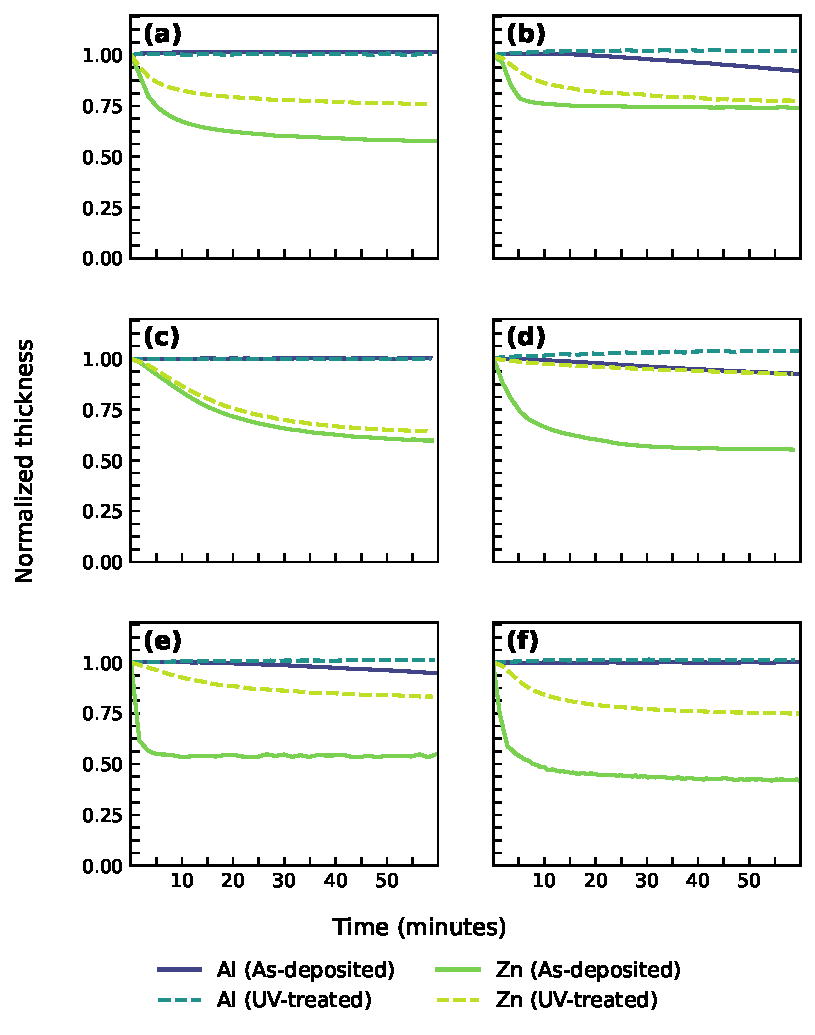
\includegraphics[width=0.75\textwidth]{Figures/air_stability_final.pdf}
    \caption{\small
    Normalized thickness change over 1 hour of air exposure for Al-based and Zn-based hybrid thin films incorporating different organic linkers. (a) MPD (methylene propanediol); (b) EG (ethylene glycol); (c) THB (trihydroxybenzene); (d) BTY (1,4-butynediol); (e) DHB (dihydroxybutene); (f) CB (cis-butenediol).
    Solid lines represent as-deposited films, while dashed lines correspond to UV-treated films. Aluminum-based (Al) and zinc-based (Zn) films are distinguished by color. Thickness values were normalized to the initial thickness at time zero.
    }
    \label{fig:air_stability}
\end{figure}


\subsection{Developer Compatibility and Patterning Contrast}

Chemical robustness and developer compatibility were assessed by immersing hybrid films in DI water, anhydrous organic solvents (acetone, toluene, chloroform), and dilute aqueous developers (\SI{0.01}{\molar} HCl and \SI{0.01}{\molar} KOH) for \SI{1}{\hour}. Post-treatment film thicknesses and refractive indices were analyzed by spectroscopic ellipsometry.

Zincone films showed extreme sensitivity, undergoing rapid dissolution in aqueous environments and substantial thickness loss in organic solvents. This severe instability likely results from facile hydrolytic cleavage of Zn--O--C linkages upon exposure to moisture or polar solvents~\cite{King2009}. While UV pretreatment modestly improved handling stability, the intrinsic chemical fragility of zincones limited their applicability for lithographic purposes.

Alucone films exhibited considerably greater robustness. As-deposited alucones experienced modest thickness decreases (\SIrange{10}{20}{\percent}) in DI water, indicative of partial hydrolysis. Organic solvent immersion generally resulted in minor thickness increases and refractive index reductions, suggesting limited solvent penetration and the formation of porous microstructures within the films~\cite{Vemuri2008}. UV-treated alucones displayed significantly enhanced chemical resistance, retaining both thickness and refractive indices after immersion in all tested solvents and aqueous solutions, reflecting the densified and crosslinked network structures induced by UV irradiation.

Three visualizations are shown for films incorporating trimethylaluminum (TMA) and diethylzinc (DEZ) as the inorganic components: heatmaps, grouped bar plots with solvents on the x-axis, and grouped bar plots with organic linkers on the x-axis. Organic linkers are ordered based on chemical structure: EG (ethylene glycol), CB (cis-butenediol), BTY (butynediol), THB (trihydroxybenzene), MPD (methylenepropanediol), and DHB (dihydroxybutene). Exposure conditions are ordered logically from aqueous (0.01 M HCl, 0.1 M KOH, Water, Ethanol), to polar aprotic (Acetone), and finally nonpolar solvents (Chloroform, Toluene). Colors correspond to the exposure condition based on the Viridis colormap. The y-axis is fixed across all plots to enable direct visual comparison of stability between TMA- and DEZ-based hybrid films.

Both \SI{0.01}{\molar} KOH and \SI{0.01}{\molar} HCl were able to fully remove films upon prolonged immersion. However, due to its aggressive etching behavior toward silicon substrates and associated risks of pattern undercutting, KOH was excluded from subsequent lithographic development considerations~\cite{Horie2010}. HCl provided selective and controlled dissolution of unexposed regions via protonation and hydrolysis of metal--O--C bonds, making it the optimal developer choice.

Short-time immersion tests in \SI{0.01}{\molar} HCl demonstrated high chemical contrast between UV-treated and as-deposited alucone films. UV-treated alucones exhibited substantially delayed dissolution rates, highlighting their suitability for high-resolution lithographic applications. This pronounced chemical contrast directly informed the selection of alucone-based materials for subsequent electron-beam lithography (EBL) studies.




\begin{figure}[H]
  \centering

  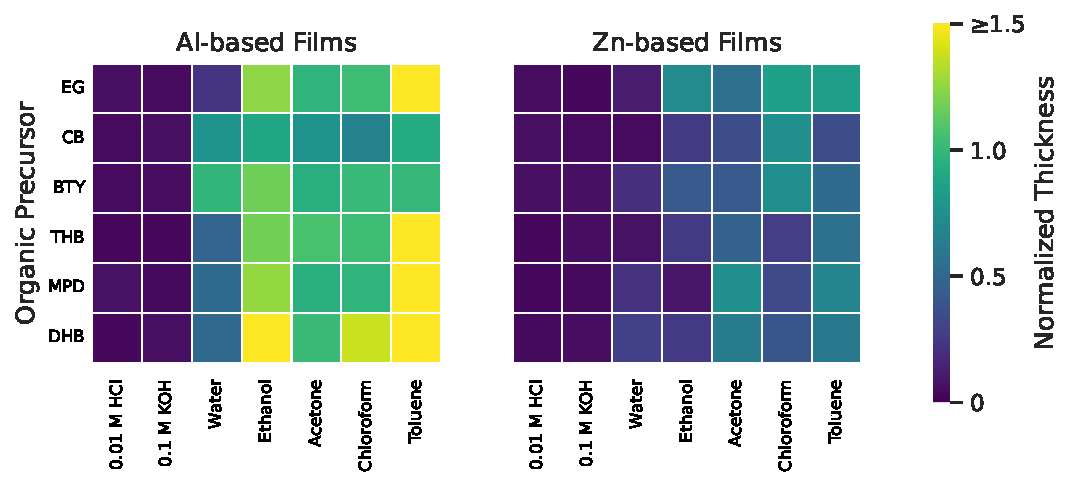
\includegraphics[width=0.9\textwidth]{Figures/Fig4a_Heatmap_EtchStability.pdf}
  \vspace{1em}

  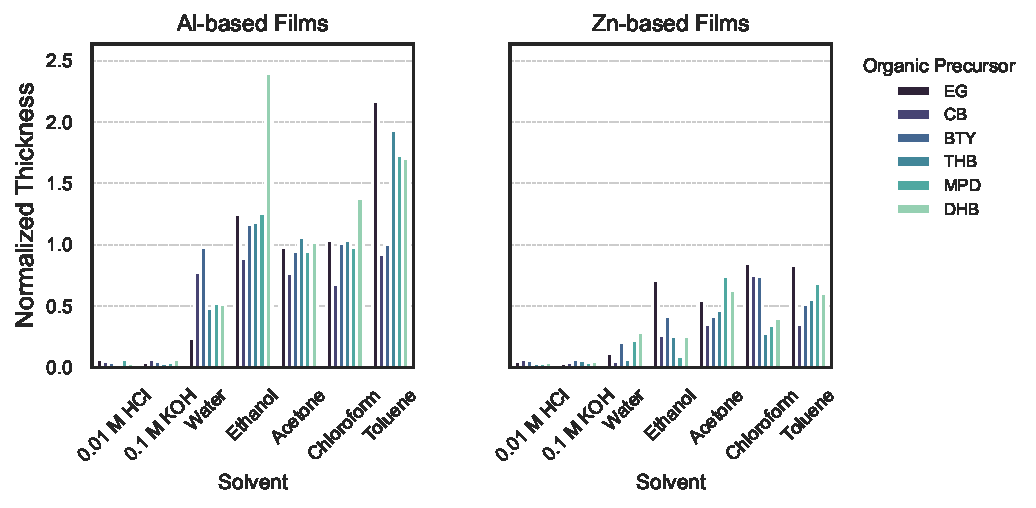
\includegraphics[width=0.9\textwidth]{Figures/Fig4b_Barplot_EtchStability.pdf}
  \vspace{1em}

  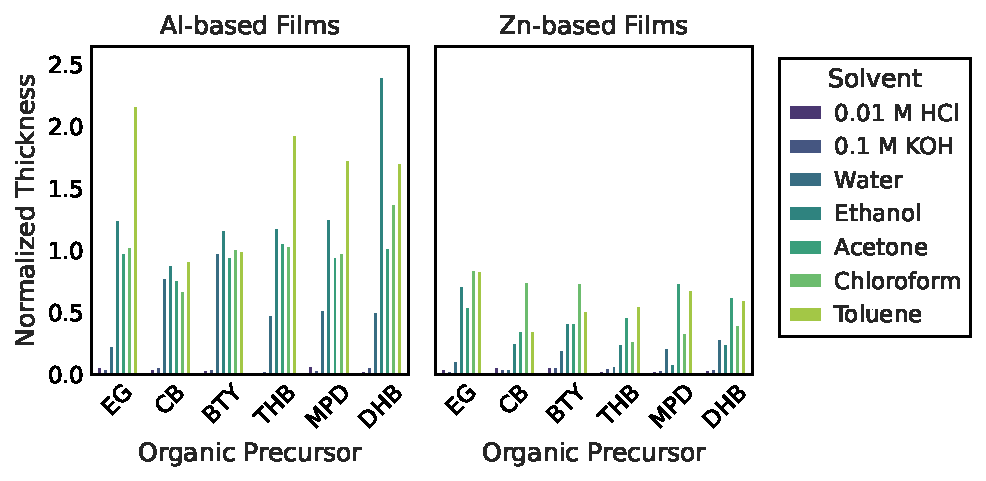
\includegraphics[width=0.9\textwidth]{Figures/Fig4c_BarplotOrganicGroupedBySolvent.pdf}

  \caption{
    Normalized thickness of as-deposited hybrid films after \SI{1}{\hour} solvent immersion, shown using three complementary visualization formats:
    \textbf{(a)} heatmaps of organic linker vs. solvent for Zn- and Al-based hybrid films (DEZ and TMA precursors, respectively);
    \textbf{(b)} grouped bar charts with solvents on the x-axis and organic linkers grouped by color; and
    \textbf{(c)} grouped bar charts with organic linkers on the x-axis and solvents grouped by color.
    Organic linkers are ordered by chemical structure: EG (ethylene glycol), CB (cis-butenediol), BTY (butynediol), THB (trihydroxybenzene), MPD (methylenepropanediol), and DHB (dihydroxybutene).
    Solvents are ordered from aqueous (\SI{0.01}{\molar} HCl, \SI{0.1}{\molar} KOH, water, ethanol) to polar aprotic (acetone), and nonpolar (chloroform, toluene).
  }
  \label{fig:developer_visualization_comparison}
\end{figure}




\subsection{Selection of Lead Materials for Advanced Characterization}

The results of air stability and aqueous compatibility screening guided the selection of alucone materials for deeper structural investigation using FTIR and XPS. These analyses were aimed at identifying systems that undergo meaningful chemical transformation upon UV exposure and show promise for patterning applications requiring environmental robustness.

Zincone films were excluded early due to their pronounced chemical instability under both ambient and aqueous conditions. Their susceptibility to rapid hydrolysis, alongside concerns over zinc volatility and contamination under vacuum conditions, rendered them unsuitable for further development~\cite{Richey2019}.

In contrast, alucone films displayed markedly greater stability, with significant differences based on the organic linker chemistry. Films deposited using 1,4-butynediol (BTY) exhibited high and consistent growth per cycle (\SI{\sim 6}{\angstrom\per\cycle}) and demonstrated clear UV-induced changes in both FTIR and XPS spectra. These changes included the loss of hydroxyl signatures, appearance of conjugated C=C and C=O features, and suppression of hydrolysis, suggesting robust photochemical crosslinking. As a result, BTY-based alucones were prioritized for further characterization and subsequent lithographic evaluation.

Alucones synthesized with 1,3,4-trihydroxybenzene (THB) showed relatively high stability even without UV treatment. Despite this intrinsic robustness, FTIR and XPS analyses revealed only subtle changes upon UV exposure, with limited evidence of significant crosslinking or network reorganization. The absence of clear UV-induced structural transformation, combined with modest aqueous degradation, led to the decision not to pursue THB-based films further for electron-beam lithography. However, their aromatic structure and partial resistance to degradation justified their inclusion in this study as a comparative system for extended spectroscopic characterization.

Other linkers, including cis-2-butene-1,4-diol (CB) and 2-methylene-1,3-propanediol (MPD), were deprioritized. CB-based films showed moderate UV-induced stabilization but did not match the performance or crosslinking response of BTY. MPD-based films exhibited minimal change upon UV exposure, reflecting limited photochemical activity and poor retention under aqueous conditions.

In summary, BTY- and THB-based alucone films were selected as lead candidates for advanced FTIR and XPS characterization. BTY was taken forward for subsequent lithographic evaluation due to its robust UV response and structural transformation. THB was retained as a chemically stable, aromatic control to better understand how phenolic structures influence hybrid film behavior and to probe the boundaries of UV-driven network modification.




\subsection{FTIR Analysis: UV-Induced Crosslinking and Network Densification}

Fourier-transform infrared (FTIR) spectroscopy was used to investigate the chemical and structural changes induced by ultraviolet (UV) exposure (\SI{254}{\nano\meter}) in TMA–BTY alucone films. Spectra collected before and after UV treatment reveal distinct modifications in vibrational modes associated with hydroxyl, carbon–carbon, and metal–oxygen bonding environments, offering mechanistic insight into UV-induced crosslinking and network densification (Figure~\ref{fig:ftir}).

The as-deposited films exhibit broad O–H stretching bands centered near 3622 and 3232~\si{\per\centi\meter}, attributed to free and hydrogen-bonded hydroxyl groups, respectively. These features are substantially diminished after UV exposure, indicating effective consumption of terminal –OH groups through condensation, elimination, or secondary reactions with photochemically activated species~\cite{REF}. This aligns with the observed disappearance of –OH signatures in post-UV XPS and confirms densification through hydroxyl removal.

A key transformation is the sharpening and intensification of the band at \SI{1612}{\per\centi\meter}, assigned to C=C stretching vibrations. This suggests the formation of conjugated or aromatic carbon domains, likely arising from cycloaddition or radical-mediated rearrangement of BTY’s internal alkyne units. Such transformations imply the development of more rigid, crosslinked structures through UV-activated coupling or cyclization pathways. Notably, direct observation of C≡C stretching modes was hindered by overlapping environmental CO$_2$ features, but the C=C evolution provides indirect confirmation of alkyne conversion.

In the fingerprint region, prominent vibrations associated with the Al–O–C backbone appear between \SIrange{1200}{800}{\per\centi\meter}, including sharp peaks near 1132, 1063, and 1012~\si{\per\centi\meter}, as well as broader modes below 700~\si{\per\centi\meter}. After UV treatment, these bands exhibit narrowing and increased definition, consistent with enhanced structural order and reduced vibrational freedom. Sharpening of Al–O bending modes at 579 and 557~\si{\per\centi\meter} further supports increased crosslink density and stabilization of the hybrid network.

Overall, these spectral changes strongly support a model in which UV irradiation removes labile hydroxyl groups, activates alkyne–alkyne or alkyne–hydroxyl coupling, and promotes structural rearrangement into conjugated or partially aromatic domains. These processes reduce network free volume, enhance cohesion, and suppress hydrolytic reactivity, explaining the dramatic improvements in film stability observed under aqueous and developer exposure.

\begin{figure}[ht]
  \centering
  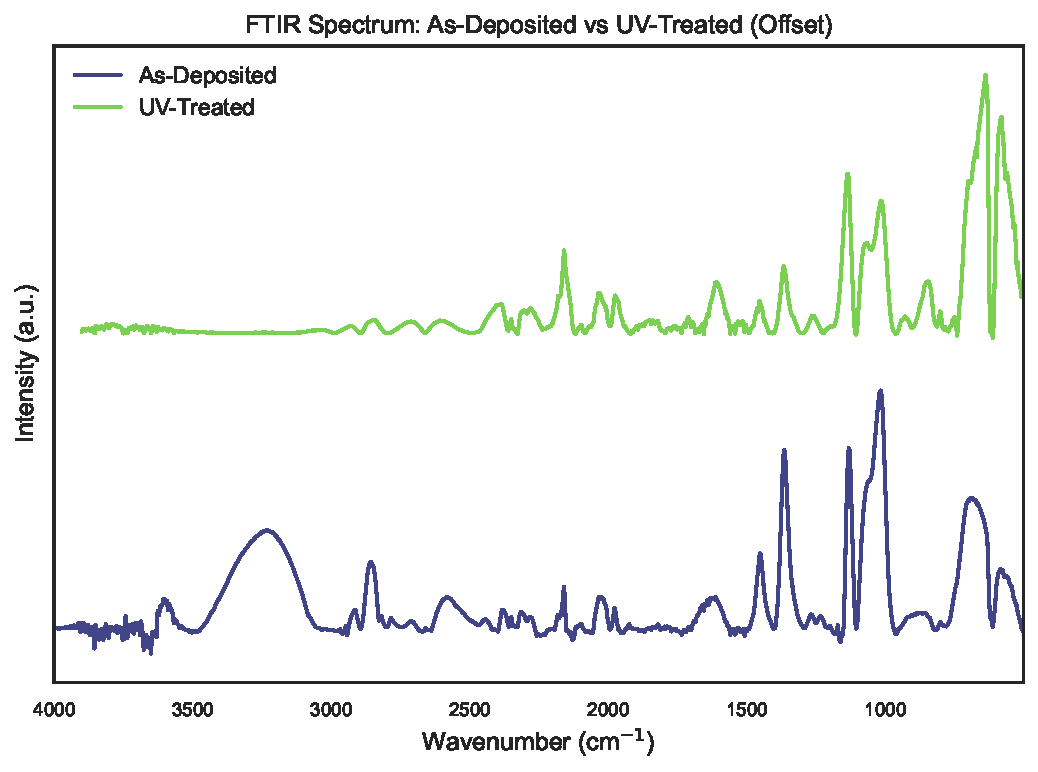
\includegraphics[width=0.75\textwidth]{Figures/Fig3a_FTIR_Offset.pdf}
  \caption{FTIR spectra of TMA–BTY alucone films before and after UV irradiation at 254~nm. Notable changes include disappearance of O–H stretching bands (3622 and 3232~\si{\per\centi\meter}), intensification and sharpening of C=C stretching near 1612~\si{\per\centi\meter}, and increased definition of Al–O–C and Al–O bending modes in the fingerprint region, consistent with UV-induced crosslinking and structural densification.}
  \label{fig:ftir}
\end{figure}


\subsection{XPS Analysis of Bonding Environments and Stability}

X-ray photoelectron spectroscopy (XPS) was employed to examine chemical bonding environments in BTY-based alucone films (TMA–BTY), providing insight into UV-induced structural transformations and their impact on hydrolytic stability. High-resolution spectra of the C~1s, O~1s, and Al~2p regions were analyzed for as-deposited, water-exposed, and UV+water-exposed samples (Figure~\ref{fig:xps_spectra}).

In the Al~2p region, all samples exhibit a primary peak centered near 74.6~eV, characteristic of Al–O–C bonding environments within alucone networks~\cite{REF}. The as-deposited film shows a single symmetric peak, while the water-exposed sample develops a subtle lower-binding-energy shoulder, indicative of partial hydrolysis and the formation of Al–O–Al or Al–OH species. The UV+water sample retains a symmetric Al~2p profile similar to the pristine film, suggesting that UV treatment suppresses hydrolytic transformation and preserves Al–O–C connectivity.

O~1s spectra reinforce this interpretation. The as-deposited film exhibits dominant Al–O–C contributions near 532~eV, with minor signals from hydroxyl groups. After water exposure, the O~1s peak broadens and shifts slightly, consistent with increased hydroxyl content and framework disruption. In contrast, the UV+water sample maintains a narrower, more symmetric O~1s envelope, consistent with limited hydrolysis and retention of the hybrid structure.

C~1s spectra show the most pronounced UV-dependent differences. The as-deposited film exhibits distinct contributions from aliphatic C–C/C–H, C–O, and a minor oxidized component. Water exposure leads to carbon depletion and a relative increase in C=O and carbonate signals, reflecting cleavage and oxidation of the organic linker. The UV+water-exposed sample retains a higher proportion of aliphatic and C–O carbon species, with attenuated oxidized contributions, indicating protection of the organic matrix.

These qualitative assessments are supported by quantitative atomic composition data (Table~\ref{tab:xps-renormalized}). After water exposure, oxygen content increases markedly from 32.9\% to 56.0\%, while carbon drops from 55.6\% to 18.6\%, consistent with organic degradation and hydration of the Al–O framework. In the UV+water-exposed sample, the oxygen content is moderated (42.5\%), and carbon is partially preserved (41.7\%), confirming that UV exposure imparts significant protection against hydrolytic attack. Aluminum content increases in both exposed samples due to relative loss of carbon and surface enrichment of inorganic species.

Together, these results confirm that UV irradiation reduces the density of hydrolysis-prone sites and stabilizes both organic and inorganic bonding environments. By suppressing Al–O–C cleavage and oxidation of the organic linker, UV-treated BTY-based alucones retain structural integrity and resist aqueous degradation, in stark contrast to their unexposed counterparts.


\begin{figure}[H]
  \centering
  \includegraphics[width=0.95\textwidth]{Figures/BTY_XPS_Final_Publication.pdf}
  \caption{High-resolution XPS spectra of BTY-based alucone films showing the evolution of chemical environments in the C~1s (left), O~1s (middle), and Al~2p (right) regions across as-deposited, water-exposed, and UV+water-exposed samples. Colored fits represent individual peak components; black crosses show experimental data.}
  \label{fig:xps_spectra}
\end{figure}

\begin{figure}[H]
  \centering
  \includegraphics[width=0.95\textwidth]{Figures/THB_XPS_Final_Publication.pdf}
  \caption{High-resolution XPS spectra of BTY-based alucone films showing the evolution of chemical environments in the C~1s (left), O~1s (middle), and Al~2p (right) regions across as-deposited, water-exposed, and UV+water-exposed samples. Colored fits represent individual peak components; black crosses show experimental data.}
  \label{fig:xps_spectra}
\end{figure}


\subsection{XPS Analysis of Bonding Environments and Stability}

X-ray photoelectron spectroscopy (XPS) was employed to examine chemical bonding environments in BTY-based alucone films (TMA–BTY), providing insight into UV-induced structural transformations and their impact on hydrolytic stability. High-resolution spectra of the C~1s, O~1s, and Al~2p regions were analyzed for as-deposited, water-exposed, and UV+water-exposed samples (Figure~\ref{fig:xps_spectra}).

In the Al~2p region, all samples exhibit a primary peak centered near 74.6~eV, characteristic of Al–O–C bonding environments within alucone networks~\cite{REF}. The as-deposited film shows a single symmetric peak, while the water-exposed sample develops a subtle lower-binding-energy shoulder, indicative of partial hydrolysis and the formation of Al–O–Al or Al–OH species. The UV+water sample retains a symmetric Al~2p profile similar to the pristine film, suggesting that UV treatment suppresses hydrolytic transformation and preserves Al–O–C connectivity.

O~1s spectra reinforce this interpretation. The as-deposited film exhibits dominant Al–O–C contributions near 532~eV, with minor signals from hydroxyl groups. After water exposure, the O~1s peak broadens and shifts slightly, consistent with increased hydroxyl content and framework disruption. In contrast, the UV+water sample maintains a narrower, more symmetric O~1s envelope, consistent with limited hydrolysis and retention of the hybrid structure.

C~1s spectra show the most pronounced UV-dependent differences. The as-deposited film exhibits distinct contributions from aliphatic C–C/C–H, C–O, and a minor oxidized component. Water exposure leads to carbon depletion and a relative increase in C=O and carbonate signals, reflecting cleavage and oxidation of the organic linker. The UV+water-exposed sample retains a higher proportion of aliphatic and C–O carbon species, with attenuated oxidized contributions, indicating protection of the organic matrix.

These qualitative assessments are supported by quantitative atomic composition data (Table~\ref{tab:xps-renormalized}). After water exposure, oxygen content increases markedly from 32.9\% to 56.0\%, while carbon drops from 55.6\% to 18.6\%, consistent with organic degradation and hydration of the Al–O framework. In the UV+water-exposed sample, the oxygen content is moderated (42.5\%), and carbon is partially preserved (41.7\%), confirming that UV exposure imparts significant protection against hydrolytic attack. Aluminum content increases in both exposed samples due to relative loss of carbon and surface enrichment of inorganic species.

Together, these results confirm that UV irradiation reduces the density of hydrolysis-prone sites and stabilizes both organic and inorganic bonding environments. By suppressing Al–O–C cleavage and oxidation of the organic linker, UV-treated BTY-based alucones retain structural integrity and resist aqueous degradation, in stark contrast to their unexposed counterparts.


\begin{figure}[H]
  \centering
  \includegraphics[width=0.95\textwidth]{Figures/BTY_XPS_Final_Publication.pdf}
  \caption{High-resolution XPS spectra of BTY-based alucone films showing the evolution of chemical environments in the C~1s (left), O~1s (middle), and Al~2p (right) regions across as-deposited, water-exposed, and UV+water-exposed samples. Colored fits represent individual peak components; black crosses show experimental data.}
  \label{fig:xps_spectra}
\end{figure}



  \begin{table}[H]
  \centering
  \caption{Renormalized atomic \% for O, C, and Al (omitting minor contaminants) in TMA–BTY alucone films.}
  \label{tab:xps-renormalized}
  \begin{tabular}{l c c c}
    \toprule
    \textbf{Sample} & \textbf{O [\%]} & \textbf{C [\%]} & \textbf{Al [\%]} \\
    \midrule
    As-Deposited       & 32.9 & 55.6 & 11.5 \\
    \midrule[0.8pt]
    H$_2$O-Exposed     & 56.0 & 18.6 & 25.4 \\
    \midrule[0.8pt]
    H$_2$O + UV        & 42.5 & 41.7 & 15.7 \\
    \midrule[0.8pt]
    \textbf{Ideal}     & 30.0 & 60.0 & 10.0 \\
    \bottomrule
  \end{tabular}
\end{table}


\subsection{XPS Analysis of Bonding Environments and Stability}

X-ray photoelectron spectroscopy (XPS) was employed to examine chemical bonding environments in THB-based alucone films (TMA–THB), providing insight into UV-induced structural transformations and their impact on hydrolytic stability. High-resolution spectra of the C~1s, O~1s, and Al~2p regions were analyzed for as-deposited, water-exposed, and UV+water-exposed samples (Figure~\ref{fig:xps_spectra}).

In the Al~2p region, all THB-based samples exhibit a primary peak centered near 74.6~eV, characteristic of Al–O–C bonding environments within alucone networks~\cite{REF}. The as-deposited film shows a single symmetric peak, while the water-exposed sample develops a noticeable shoulder at lower binding energy (~73.8 eV), indicating significant hydrolysis with formation of Al–O–Al or Al–OH species. In contrast, the UV+water sample maintains a more symmetric Al~2p profile with minimal shoulder development, suggesting that UV pre-treatment effectively suppresses hydrolytic transformation of Al–O–C bonds.

The O~1s spectra provide complementary evidence of the UV-induced stabilization mechanism. The as-deposited film exhibits a primary peak at ~532.0 eV assigned to Al–O–C linkages with a minor contribution from hydroxyl groups at higher binding energy (~533.2 eV). Water exposure causes pronounced peak broadening toward lower binding energy (~530.8 eV), consistent with increased Al–O–Al network formation and framework disruption. Remarkably, the UV+water sample maintains an O~1s profile closer to the as-deposited state, with reduced contributions from the lower binding energy species, confirming the preservation of hybrid organic-inorganic connectivity.

The C~1s spectra reveal the most dramatic differences between treatment conditions. The as-deposited THB-based film displays multiple carbon environments: aromatic/aliphatic C–C/C–H (~284.8 eV), C–O (~286.2 eV), and minor oxidized components (C=O/O–C=O at ~288-289 eV). Water exposure leads to substantial carbon loss with a relative increase in oxidized carbon species, reflecting degradation of the organic linker. The UV+water-treated sample maintains significantly higher carbon content with a spectral profile closer to the as-deposited film, particularly preserving the C–O component associated with intact Al–O–C bonds.

This preservation of chemical environments in UV-treated THB-alucones suggests a fundamental transformation that protects both the organic and inorganic components from hydrolytic attack. By comparison, similarly prepared BTY-based alucones show analogous stabilization patterns, though the aromatic THB linker appears to provide enhanced resistance to oxidative degradation after UV treatment, as evidenced by better preservation of C–C and C–O bonding environments.

The spectroscopic evidence indicates that UV irradiation induces crosslinking within the hybrid framework while reducing the density of hydrolysis-prone sites. This photochemical transformation effectively stabilizes both the aluminum coordination environment and the organic linker structure, enabling THB-based alucones to maintain structural integrity under aqueous conditions that rapidly degrade their non-irradiated counterparts.

\begin{figure}[H]
  \centering
  \includegraphics[width=0.95\textwidth]{Figures/THB_XPS_Final_Publication.pdf}
  \caption{High-resolution XPS spectra of THB-based alucone films showing the evolution of chemical environments in the C~1s (left), O~1s (middle), and Al~2p (right) regions across as-deposited, water-exposed, and UV+water-exposed samples. Colored areas represent individual peak components; black markers show experimental data points.}
  \label{fig:xps_spectra}
\end{figure}


\begin{table}[H]
\centering
\caption{Renormalized atomic \% for O, C, and Al (mean ± standard deviation) for TMA–BTY and TMA–THB alucone films across treatments.}
\label{tab:xps-bty-thb-corrected-final}
\begin{tabular}{l c c c c c c}
\toprule
\multirow{2}{*}{\textbf{Treatment}} & \multicolumn{3}{c}{\textbf{BTY [\%]}} & \multicolumn{3}{c}{\textbf{THB [\%]}} \\
\cmidrule(lr){2-4}\cmidrule(lr){5-7}
 & O & C & Al & O & C & Al \\
\midrule
As-Deposited & 29.2 ± 0.8 & 58.9 ± 0.4 & 11.9 ± 0.5 & 42.8 ± 1.8 & 25.9 ± 2.4 & 31.3 ± 0.6 \\
H$_2$O-Exposed & 56.0 ± 0.5 & 18.6 ± 0.5 & 25.3 ± 0.3 & 50.2 ± 0.6 & 17.2 ± 1.6 & 32.6 ± 1.0 \\
H$_2$O + UV & 32.9 ± 1.2 & 55.6 ± 1.5 & 11.5 ± 0.4 & 46.8 ± 1.0 & 20.2 ± 1.2 & 33.0 ± 0.1 \\
\midrule
Ideal (MLD) & 20.0 & 70.0 & 10.0 & 23.1 & 69.2 & 7.7 \\
\bottomrule
\end{tabular}
\end{table}

\subsection{Mechanistic Insight into UV-Induced Stabilization}

The combined spectroscopic evidence from FTIR and XPS analyses supports a detailed mechanistic model for UV-induced structural transformations and stabilization in BTY-based alucone (TMA–BTY) films. Figure~\ref{fig:structure_evolution} schematically summarizes the proposed structural evolution, illustrating key changes from the as-deposited state through UV exposure and subsequent aqueous degradation.

As-deposited alucone films are composed primarily of repeating \ce{Al–O–CH2–C#C–CH2–O–Al} units, formed through alternating reactions of trimethylaluminum (TMA) and 1,4-butynediol (BTY). FTIR spectra reveal residual hydroxyl stretching bands near 3622 and 3232~\si{\per\centi\meter}, indicative of unreacted –OH groups from the diol. These likely arise from steric constraints or incomplete surface reactions during deposition~\cite{REF}.

Upon UV irradiation at \SI{254}{\nano\meter}, the organic linker undergoes substantial photochemical activation. The most pronounced FTIR change is the intensification of the C=C stretching mode near \SI{1612}{\per\centi\meter}, consistent with alkyne rearrangement or cycloaddition reactions that generate conjugated or aromatic domains. These processes likely proceed via [2+2] or radical-mediated mechanisms, producing rigid, crosslinked structures that increase film density and reduce chemical reactivity. Simultaneously, FTIR shows a marked reduction in hydroxyl-related absorptions, indicating consumption of –OH groups through dehydration, elimination, or ether/ester formation.

XPS measurements corroborate this UV-induced stabilization. C~1s spectra show reduced contributions from hydroxyl- and carbonate-associated carbon, alongside increased signals for aliphatic or conjugated C–C environments. These features suggest conversion of C–OH into C=O and extended π-systems, including possible quinone-like moieties. Al~2p and O~1s regions remain largely unchanged after UV+H$_2$O exposure, indicating that Al–O–C bonds are preserved and hydrolysis-induced Al–O–Al formation is suppressed.

By contrast, non-irradiated films exposed to water undergo substantial hydrolytic breakdown. Increased Al–O–Al content, oxidized carbon, and carbonate formation point to cleavage of Al–O–C bonds and oxidative degradation of the organic backbone. This results in a porous alumina-like matrix and significantly diminished chemical robustness.

Together, these observations reveal that UV irradiation promotes irreversible transformations in the hybrid film structure: removal of labile –OH groups, formation of stable conjugated domains, and suppression of hydrolysis-prone sites. This leads to chemically and mechanically resilient networks capable of withstanding aqueous or developer exposure—an essential property for hybrid photoresists in advanced lithographic processes.

\begin{figure}[ht]
  \centering
  \includegraphics[width=0.85\textwidth]{figures/structure_evolution.pdf}
  \caption{Proposed structural evolution and chemical transformations of BTY-based alucone films during UV irradiation and subsequent hydrolytic exposure: (a) as-deposited film containing residual hydroxyl groups and isolated alkyne linkages, (b) UV-treated film exhibiting crosslinked conjugated structures and reduced hydroxyl content, and (c) hydrolytically degraded film without UV treatment, illustrating extensive bond cleavage and porous structure formation.}
  \label{fig:structure_evolution}
\end{figure}



\subsection{Electron-Beam Lithography Studies}

To evaluate the lithographic potential of BTY-based alucone films, electron-beam lithography (EBL) experiments were conducted using a JEOL JBX-6300FS system operating at \SI{100}{\kilo\volt}. This work focused exclusively on alucones synthesized from 1,4-butynediol (BTY), given their demonstrated structural robustness, pronounced UV-induced stabilization, and strong crosslinking response observed in FTIR and XPS analyses.

EBL exposure was performed on both as-deposited and UV flood-exposed films to directly assess the effect of UV pretreatment on electron-beam response. Dose matrices spanning \SIrange{500}{5000}{\micro\coulomb\per\centi\meter\squared} were patterned to explore contrast, resolution, and dose-to-clear behavior. A representative dose matrix layout is shown in Figure~\ref{fig:dose_matrix} (placeholder).

Initial results suggest a negative-tone response, in which exposed regions become less soluble in aqueous or acidic developers. This behavior is consistent with earlier observations of UV-induced crosslinking and densification, and suggests that BTY-based alucones can undergo similar crosslinking under e-beam irradiation. Comparing the two conditions—untreated vs. UV-pretreated—will provide insight into whether UV-induced structural transformations enhance or inhibit e-beam-induced patternability.

Subsequent analysis will include contrast curves derived from normalized remaining thickness versus dose, enabling extraction of dose-to-clear values and contrast (\(\gamma\)) parameters. High-resolution scanning electron microscopy (SEM) and atomic force microscopy (AFM) will be used to characterize line-edge roughness (LER), sidewall profiles, and resolution limits, offering deeper understanding of how crosslinked hybrid networks influence pattern fidelity.

% Placeholder for quantitative results and comparative discussion:
% - Dose-to-clear values (optimal doses identified clearly)
% - Measured contrast (\(\gamma\)) values from fitted contrast curves
% - SEM images explicitly showing resolution limits, sidewall profiles, and LER
% - AFM measurements of topography clearly illustrating pattern fidelity

These experiments are designed to correlate structural features observed in earlier FTIR and XPS characterizations with real-world lithographic performance. By comparing as-deposited and UV-treated BTY alucone films under identical EBL conditions, this study aims to clarify the role of pre-exposure crosslinking in tuning developer resistance, resolution, and contrast—key parameters in the design of high-performance hybrid resist materials.

\begin{figure}[ht]
  \centering
  \includegraphics[width=0.75\textwidth]{figures/dose_matrix_placeholder.pdf}
  \caption{Placeholder for electron-beam lithography dose-matrix patterns demonstrating exposure-dose dependence of film retention, resolution limits, and contrast for as-deposited and UV-treated BTY-based alucone films. Final figure will include labeled dose values and pattern dimensions.}
  \label{fig:dose_matrix}
\end{figure}

